\section{Linear Regression Dataset}
This task involved analyzing a dataset using linear regression techniques. 
The objective was to design a linear regression model to fit the data and make predictions based on the input features. 
This dataset does not have a specified set of features, just a set of x and y train and test values. 
The efforts in this task reflected the efforts from the Salary Dataset task, but without a specified feature set.

\subsection{Implementation Details}
The Linear Regression model was implemented using the \texttt{LinearRegression} class from the \texttt{sklearn.linear\_model} module~\cite{sklearn_linear_model}.
The training and testing datasets were loaded from the provided CSV files using Polars~\cite{polars}. 
The x and y training values were extracted from the dataset and used to fit the \texttt{LinearRegression} model.
After the training was complete, predictions were made on both the training and testing datasets and statistics were calculated to evaluate the model's performance.

\newpage
\subsubsection{Data Handling}
The dataset was read using Polars as follows:
\begin{minted}{python}
import polars as pl

train_data_location = 'dataset/Linear_Regression/train.csv'
test_data_location = 'dataset/Linear_Regression/test.csv'
train_data = pl.read_csv(train_data_location)
test_data = pl.read_csv(test_data_location)
X_train = train_data[['x']]
y_train = train_data['y']
X_test = test_data[['x']]
y_test = test_data['y']
\end{minted}

\noindent The resultant dimensions of the data arrays were:
\begin{itemize}
    \item \textbf{X\_train}: (700, 1) -- 700 samples with 1 feature (x values for training data)
    \item \textbf{y\_train}: (700,) -- 700 target values (y values for training data)
    \item \textbf{X\_test}: (300, 1) -- 300 samples with 1 feature (x values for testing data)
    \item \textbf{y\_test}: (300,) -- 300 target values (y values for testing data)
\end{itemize}

\subsubsection{Model Training}
The Linear Regression model was trained using the following code:
\begin{minted}{python}
from sklearn.linear_model import LinearRegression

model = LinearRegression()
model.fit(X_train, y_train)
y_train_pred = model.predict(X_train)
y_test_pred = model.predict(X_test)
\end{minted}

\noindent The resultant dimensions of the y\_test and y\_train prediction arrays were:
\begin{itemize}
    \item \textbf{y\_train\_pred}: (700,) -- 700 predicted y values for training data
    \item \textbf{y\_test\_pred}: (300,) -- 300 predicted y values for testing data
\end{itemize}

\newpage
\subsection{Results}
\subsubsection{Plotted Graph}

The resultant graphs of the linear regression model comparisons are shown in Figure~\ref{fig:linear_regression}.

\begin{figure}[htbp]
    \centering
    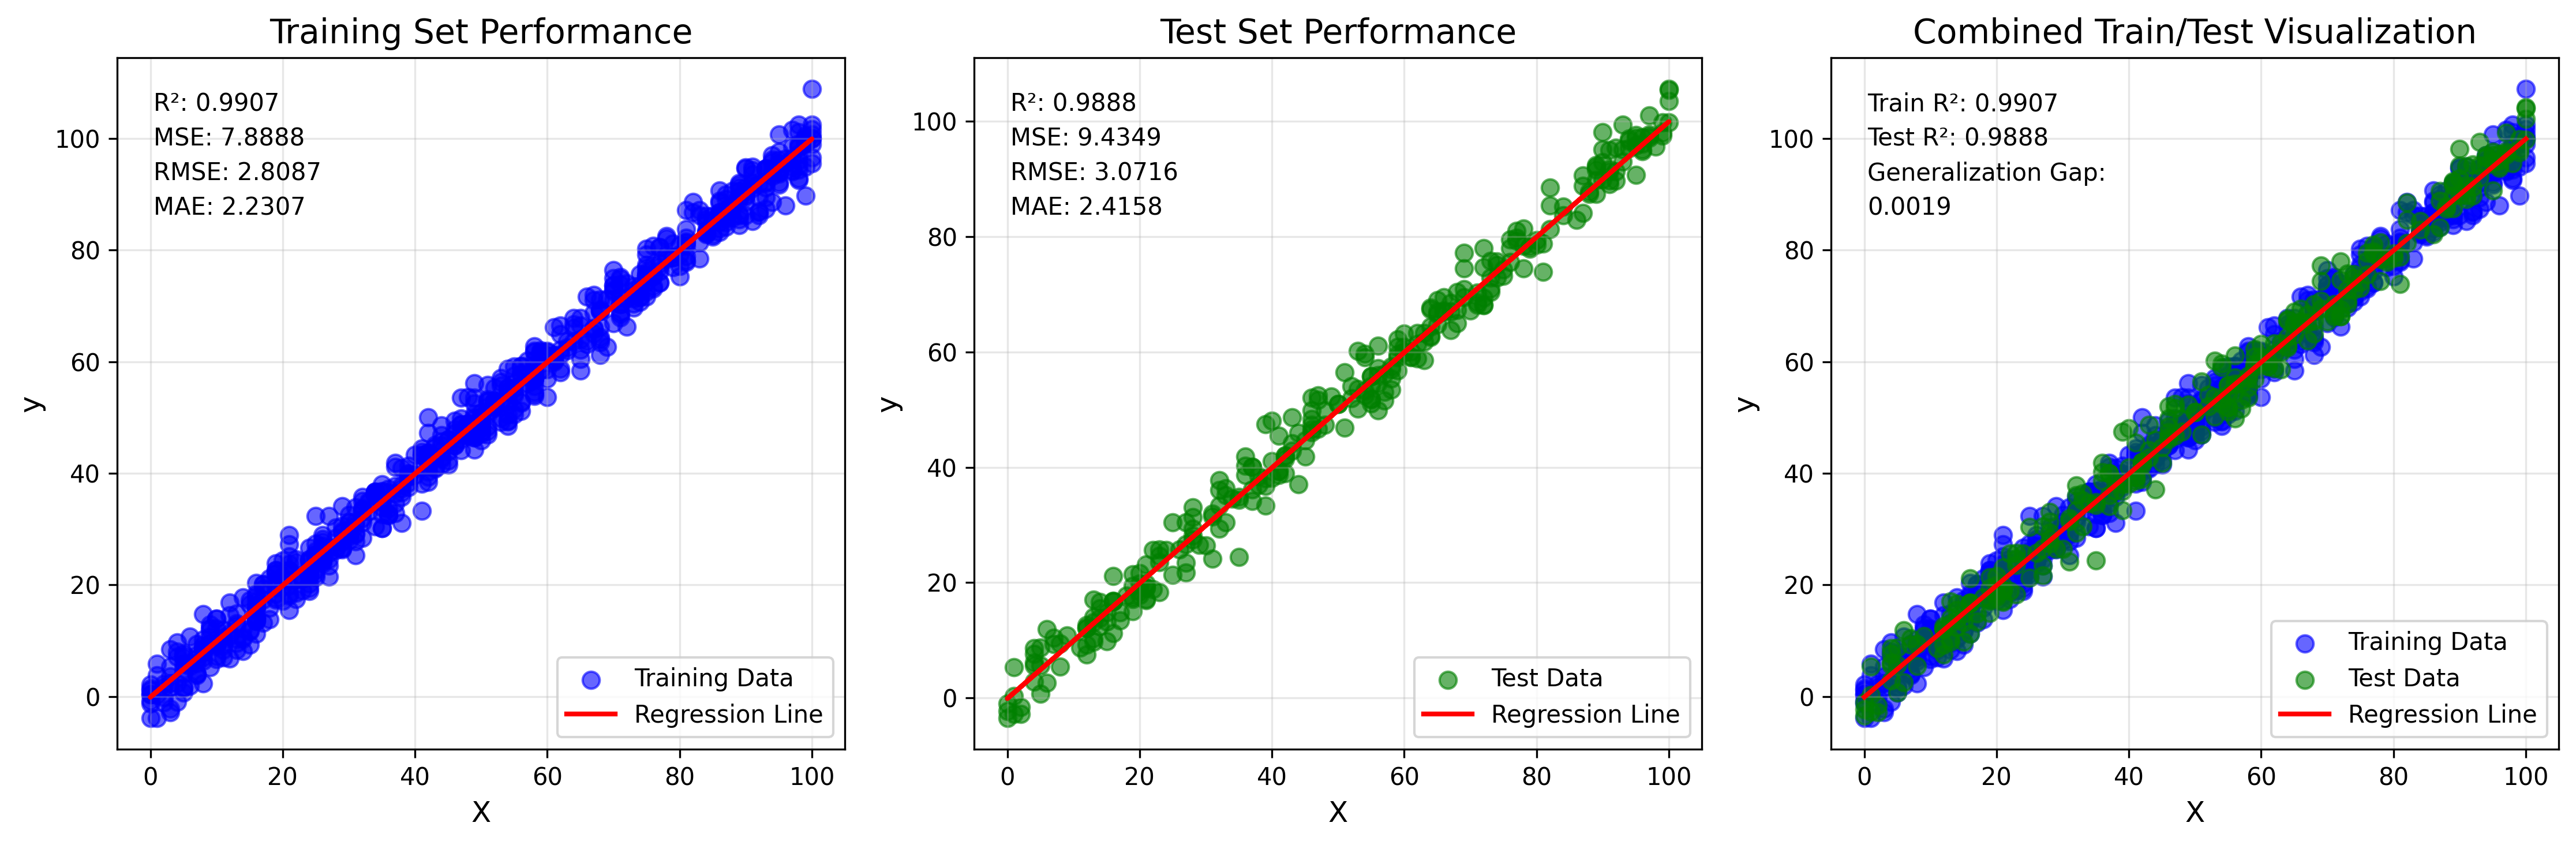
\includegraphics[width=\textwidth]{images/linear_regression_analysis_plot.png}
    \caption{Linear Regression Model Plot}\label{fig:linear_regression}
\end{figure}

\subsubsection{Analysis}
The performance of the Linear Regression model was evaluated using several metrics.
The results are summarized in Table~\ref{tab:linear_regression_results}.

% \begin{table}[htbp]
%   \centering
%   \begin{tabular}{|l|c|c|l|}
%   \hline
%   \textbf{Metric} & \textbf{Training} & \textbf{Test} & \textbf{Interpretation} \\
%   \hline
%   R² Score & 0.9907 & 0.9888 & Excellent fit, minimal overfitting \\
%   \hline
%   MSE & 7.8888 & 9.4349 & Low error, good generalization \\
%   \hline
%   RMSE & 2.8087 & 3.0716 & Root mean squared error \\
%   \hline
%   MAE & 2.2307 & 2.4158 & Average absolute error \\
%   \hline
%   \multicolumn{4}{|c|}{\textbf{Generalization Analysis}} \\
%   \hline
%   R² Difference & \multicolumn{2}{c|}{0.0019} & Model generalizes well \\
%   \hline
%   \end{tabular}
%   \caption{Linear Regression Performance Metrics and Generalization Analysis}\label{tab:linear_regression_results}
% \end{table}

\begin{table}[htbp]
    \centering
    \begin{tabular}{ || l || c || c || l || }
        \hline
        \textbf{Metric} & \textbf{Training} & \textbf{Test} & \textbf{Interpretation} \\
        \hline\hline
        R² Score & 0.9907 & 0.9888 & Excellent fit, minimal overfitting \\
        \hline
        MSE & 7.8888 & 9.4349 & Low error, good generalization \\
        \hline
        RMSE & 2.8087 & 3.0716 & Root mean squared error \\
        \hline
        MAE & 2.2307 & 2.4158 & Average absolute error \\
        \hline\hline
        \multicolumn{4}{||c||}{\textbf{Generalization Analysis}} \\
        \hline\hline
        R² Difference & \multicolumn{2}{c||}{0.0019} & Model generalizes well \\
        \hline
    \end{tabular}
    \caption{Linear Regression Performance Metrics and Generalization Analysis}\label{tab:linear_regression_results}
\end{table}

The small generalization gap~\cite{wiki_generalization_error} between the training and test R² scores (0.0019) indicates that the model generalizes well to unseen data, with minimal overfitting.
The low MSE, RMSE, and MAE values when compared to the data ranges reinforce the generalization analysis for the model's accuracy in predicting the target variable.